\documentclass[a4paper, 11pt]{report}
\setcounter{tocdepth}{4}
\setcounter{secnumdepth}{4}
\usepackage{a4}

\usepackage{pdfpages}
\usepackage[utf8]{inputenc}
\usepackage{dsfont}
\usepackage{amsmath}
\usepackage{graphicx}
\usepackage{here}
\usepackage[section]{placeins}
\usepackage[ngerman]{babel}
\usepackage[font=small,labelfont=bf,margin=\parindent,tableposition=top]{caption}
\usepackage{subcaption}

\usepackage[colorlinks, pdfpagelabels, pdfstartview = FitH, bookmarksopen = true, bookmarksnumbered = true, linkcolor = black, plainpages = false, hypertexnames = false, citecolor = black, urlcolor = blue] {hyperref}
\parindent 0pt


\title{Dokumentation der Projektarbeit - Carrera Bahn}
\author{Florian Weber - 44907}
\date{\today}

\begin{document}
\maketitle	%Deckblatt


\tableofcontents 	%Inhaltsverzeichnis
\listoffigures		%Bildverzeichnis
\newpage

\chapter{Vorwort}%TITEL ÜBERARBEITEN
	\begin{figure}[tb]
	\centering
	\includegraphics[width=0.95\textwidth]{rec/Carrerabahnroh.png}
	\caption[Überblick über die Carrera Bahn]{Überblick über die Carrera Bahn mit den Photovoltaik Modulen, der Steuerung mit dem Human Interface Device (HMI), sowie der Bahn mit den markierten Sensorpositionen.}
	\label{img:carrerakomplett}
	\end{figure}
Die Carrera Bahn ist in Abbildung \ref{img:carrerakomplett} dargestellt. Sie ermöglicht es, zwei Autos gegeneinander antreten zu lassen. Dabei kann bei jedem Auto gewählt werden, ob es automatisch fährt oder durch einen Nutzer manuell gesteuert wird. Die Energieversorgung der jeweiligen Bahn kann unabhängig davon gewählt werden. Es ist dadurch zum Beispiel möglich, als Studierender ein Auto mit Netzstrom manuell, gegen ein automatisch fahrendes Auto, welches mit Solarstrom betrieben wird, zu steuern.
 Dies soll die Chancengleichheit der zwei Energieversorgungen demonstrieren. %

\section{Zustand der Carrera Bahn vor der Projektarbeit}
Zu Beginn des Projekts ist die Carrera Bahn auf dem Stand, dass die Fahrzeuge schon konventionell sowie automatisiert betrieben werden können. Außerdem ist die Rundenzeitmessung und deren Visualisierung bereits realisiert. Bei der Energieversorgung kann zwischen Solarstrom und Netzversorgung gewählt werden.
Die Solarstromversorgung wird pro Bahn durch 2 Solarpanels und einem Tiefsetzsteller mit konstantem Dutycycle hergestellt, die Netzstromversorgung mit einem 15V Schaltnetzteil.

Die manuelle Steuerung der Fahrzeuge durch den Nutzer ist realisiert, indem die klassischen Carrera Handregler, als variablen Vorwiderstand zu den Fahrzeugen eingesetzt werden. Im automatisierten Modus ist es möglich, mit je einem 5W Potentiometer die Geschwindigkeit des langsamen Streckenabschnittes einzustellen. In dem schnellen Steckenabschnitt (dem Looping) überbrückt ein Relais diesen Potentiometer und es liegt die volle Betriebsspannung, der jeweiligen Energieversorgung am Auto an.
\newpage
\section{Probleme der vorhandenen Carrera Bahn und Zielsetzung zur Projektarbeit}
Der zuvor erwähnte Aufbau der vorhandenen Anlage vor der Projektarbeit weist einige Probleme auf:
\begin{itemize}
	\item{1.} Solarstromversorgung und Netzversorgung sind nicht chancengleich ausgeführt. (Die Netzversorgung stellt eine stabilisierte Spannungsquelle dar, die Solarstromversorgung eine unstabilisierte Quelle.)
	\item{2.} Temperaturdrift des Widerstands des Potentiometers um den Arbeitspunkt im automatisierten Modus.
	\item{3.} Framerate der Visualisierung ist zu gering, sodass diese immer die selbe Zahlensequenz nach dem Komma anzeigt.
	\item{4.} Manchmal wird durch einen Aliasingeffekt das Überfahren eines Sensors in der Bahn nicht erkannt und die Geschwindigkeit wird nicht umgeschalten. (Echtzeitfähigkeit des Betriebssystems Raspian ist nicht gegeben)
\end{itemize}
Die oben genannten Probleme sind durch ein neues Steuer-/Regelkonzept, sowie ein Mikrocontroller mit echtzeitfähiger Software gelöst.


\chapter{Funktion - Hardware}
	Im Folgenden wird der grundlegende Aufbau der Carrera Bahn nach Abschluss der Projektarbeit erklärt.

	Diese Beschreibung ist immer nur für Bahn-A, da die
	Bahn-B analog dazu funktioniert. Dazu wird immer wieder auf die Abbildung \ref{img:signalfluss}, sowie auf die \\Abbildung
	\ref{img:carrerakomplett} Bezug genommen.\\
	Die Sensoren in den Schienen teilen die Bahn in 3 Streckenabschnitte auf:
	\begin{itemize}
		\item{1.} Startlinie $\rightarrow$ Vor dem Looping
		\item{2.} Vor dem Looping $\rightarrow$ Nach dem Looping
		\item{3.} Nach dem Looping $\rightarrow$ Startlinie
	\end{itemize}
	Auf Abschnitt 1 und Abschnitt 3 wird im automatisierten Modus die mittlere Geschwindigkeit des Autos geregelt.
	Im Looping (Streckenbschnitt 2) wird die Spannung auf einen konstanten Wert geregelt.
	Die Grenze dafür ist durch die Position der Sensoren festgelegt und somit nicht variabel.
	\begin{figure}[ht]
		\centering
		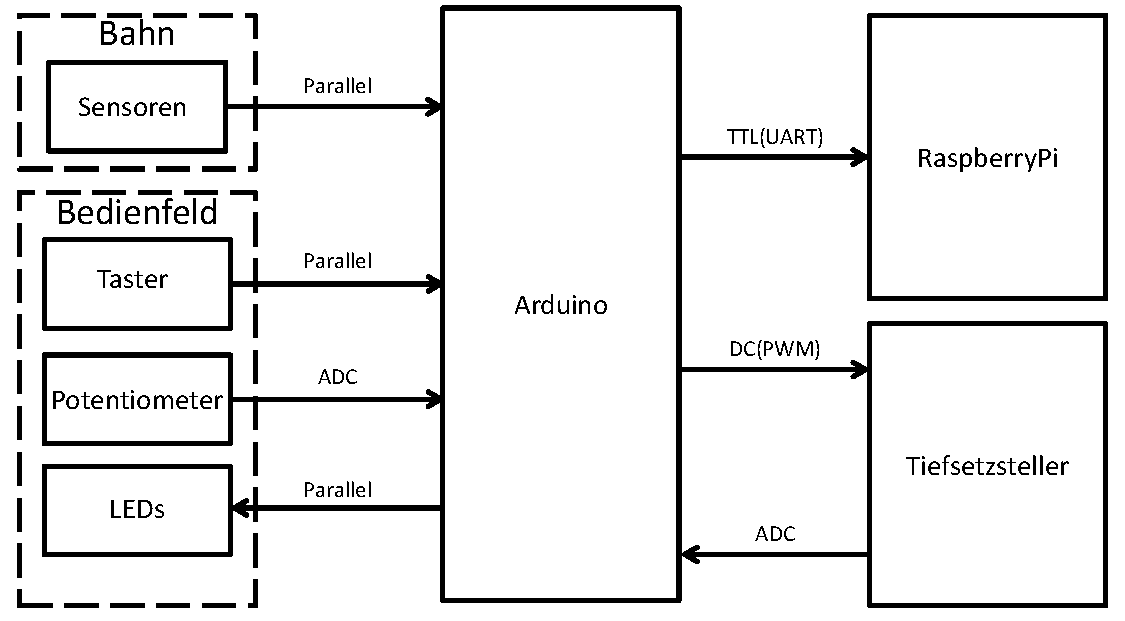
\includegraphics[width=0.85\textwidth]{rec/signalfluss.pdf}
		\caption[Signalflussbild der Steuerung]{Signalflussbild der Steuerung. \\Arduino liest Signale von Sensoren, sowie Tastern parallel aus und misst die Ausgangsspannung der Tiefsetzsteller (TSS) und Handregler. Auf Grundlage dieser Daten, generiert der Arduino die PWM Signale für die TSS und leitet die Sensordaten per Universal Asynchronous Receiver Transmitter (UART), an den RaspberryPi, zur Rundenzeitmessung weiter.}
		\label{img:signalfluss}
	\end{figure}
	In Abbildung \ref{img:signalfluss} ist eine Übersicht über den Signalfluss der Carrera Bahn dargestellt.
	Auf der Bahn stellt der Arduino das zentrale Element dar.
	Dieser liest die Sensoren in den Schienen, sowie die Taster des Human Maschine Interfaces (HMI) parallel ein und gibt die Signale der LEDs, welche den aktuellen Zustand des jeweils aktiven Modus signalisieren, parallel aus.
	Die analogen Größen (Ausgangsspannung Tiefsetzsteller (TSS), Spannung über Strommessshunt TSS, Ausgangsspannung Spannungsteiler Handregler) sind an den Analog-Digital-Wandler (ADC) des Arduinos angeschlossen.
	Der Arduino generiert außerdem die zwei PWM-Signale, die von den Tiefsetzstellern benötigt werden, über einen 8-bit Hardwaretimer.
	Dies ist genauer in Abschnitt \ref{subsec:PWM} beschrieben.
	Um eine Visualisierung zu realisieren ist ein RaspberryPi per Universal Asynchronous Receiver Transmitter (UART) seriell angebunden. Wie die anderen Kommunikationsverbindungen, ist auch diese Verbindung nur unidirektional ausgeführt.
	Die genaue Implementierung der Schnittstellen ist in den jeweiligen Kapiteln genauer beschrieben.
	\section{Sensoren}
		Wie in Abbildung \ref{img:carrerakomplett} zu sehen ist, gibt es pro Bahn 3 Sensoren. Diese sind als Gabellichtschranken ausgeführt. Sensor 0 befindet sich am Start von Bahn A, Sensor 1 vor dem Looping und Sensor 2 nach dem Looping.\\


		Sensor 0 wird ausschließlich zur Zeitmessung genutzt.
		Sensor 1 wird genutzt um ein Signal zu generieren, so dass die Steuerung das Auto im Automatik-Modus für den Looping beschleunigen kann.
		Das Signal von Sensor 2 wird schließlich genutzt um nach dem Looping wieder die langsame Geschwindigkeit zu triggern.\\
		Sensor 3 bis 5 stellen die selben Signale, analog zu Bahn A, von Bahn B bereit.

		Im manuellen Modus dienen die Sensoren nur zur Zeitmessung für die Visualisierung.

		Da die Flanke eines Sensors nur sehr kurz ist, lässt sich diese nicht per Polling ohne Aliasing Effekte digitalisieren. Stattdessen werden die Signale der Bahnsensoren durch Hardware Pin Change Interrupts (PCINT) des Arduino digitalisiert.
		Die Funktionsweise dieser PCINTs ist genauer im Abschnitt \ref{subsubsec:PCINT} erklärt
	\section{Human Human Maschine Interface}
		\begin{figure}[ht]
			\centering
			\includegraphics[width=0.95\textwidth]{rec/hid.png}
			\caption{HMI mit Arduino, RaspberryPi und TSS}

			\label{img:hid}
		\end{figure}
		Wie in Abbildung \ref{img:hid} dargestellt, besteht das Human Maschine Interface (HMI) aus 3 Wechseltaster mit Mittelstellung sowie einem Wechselschalter mit Mittelstellung.

		Der Wechselschalter ist zum Auswählen der Energieversorgung der jeweiligen Bahn. Hierbei stehen die 2 Versorgungsmöglichkeiten Solar oder Netz zur Auswahl. Ist dieser Wechselschalter in Mittelstellung, wird die Bahn nicht versorgt und das Auto steht unabhängig des gewählten Modus.
		Über Taster 0 beziehungsweise Taster 1 lässt sich der Modus der Bahn auswählen. Taster 0 steht für den manuellen Modus Von Bahn A, Taster 1 für den automatisierten. Der aktuell ausgewählte Modus wird durch die LEDs über bzw unter den Tastern signalisiert.
		Mit Taster 2 lässt sich der Regler der Bahngeschwindigkeit, genauer Sollspannung außerhalb des Loopings, auf seinen Startwert zurücksetzen.
		Global existiert noch ein weiterer Taster um die Visualisierung (Rundenzeitmessung) zurückzusetzen.
	\section{Arduino}
		Beim Arduino handelt es sich um einen Arduino Mega 2560 ADK.\\
		Dieser ist mit einem ATmega2560 der Firma Microchip bestückt.
		%warum wird ein arduino eingesetzt?
		%debug funktion
		%tacktung 16MHz
		%5v Versorgungsspannung

		Dies sind zum Beispiel die Abblockkondensatoren an der Versorgungsspannung, aber auch einen USB-Seriell Wandler, der genutzt wird, um sich Daten parallel zum Prozess an ein Terminal auszugeben.
		Letzteres lässt sich sehr gut für das Debugging nutzen.

	\section{RaspberryPi}
		Die Visualisierung ist durch ein RaspberryPi Model 3 B+ realisiert. Dieser empfängt per UART die codierten Signale der Sensoren, sowie des Tasters \glqq Reset Visualisierung \grqq (siehe Abbildung \ref{img:hid}).
		Die Visualisierung ist zu Beginn der Projektarbeit bereits vorhanden und in Form eines Python Skripts implementiert.
	\section{Tiefsetzsteller}
		Die Tiefsetzsteller fungieren als Stellglieder der Spannungsregelungen der Schienen (innerer Regelkreis der Kaskadenregelung).
		Dabei sind die Bahnen jeweils direkt an die Ausgänge der beiden TSS angeschlossen.
	  Der Arduino generiert die zwei PWM Signal für die TSS.
		Die Ausgangsspannung der TSS wird vom Arduino gemessen und durch die PWM Signale auf ihre aktuellen Sollwerte geregelt.
		Die Ausgangsspannung eines TSS ist lediglich durch die Leerlaufspannung eines PV-Strangs %HIEEEEEER ZAHLENWERT EINTRAGEN EVT MESSEN !!!
		nach oben hin begrenzt.
		Da diese größer sein kann wie die Referenzspannung des ADC (interne Referenzspannung von 2.56V), wird sie über einen Spannungsteiler angepasst und kann damit auf einen Kanal des Analog-Digital-Wandlers des Mikrocontrollers geführt werden.
		Desweiteren ist über ein Shunt eine Strommessung realisiert.
		Der Wert liegt zwar im Arduino digital vor, wird allerdings nicht weiter
		verarbeitet und ist lediglich für weiterführende Projekte gedacht.

\chapter{Software}
	\section{RaspberryPi}

		Bei der Software, die auf dem RaspberryPi ausgeführt wird, handelt es sich um ein Python Skript.
		Das Script bekommt die Signale der Sensoren, sowie des Tasters \glqq Reset Visualisierung \grqq, über die serielle Schnittstelle \glqq ttyAMA0 \grqq, gesendet und führt eine Rundenzeitmessung je Bahn durch.
		Diese Zeitmessung wird auf dem Bildschirm angezeigt.
		Zum Rendern der schrften sowie dem Hintergrundbild, ist die Open Source Bibliothek \glqq PyGame\grqq in Verwendung.
		Das Bild ist separiert in einen Hintergrund und einem Block der den dynamischen Inhalt der Rundenzeitmessung enthält.
		Um die Framerate entgegen der Version aus einer vorherigen Arbeit zu steigern, wird lediglich der dynamische Inhalt framweise neu gerendert.
	\section{Arduino}
		Die Software des Arduinos ist nicht in der Arduino Entwicklungsumgebung geschrieben, da dies einen direkten Zugriff auf die Hardware erschwert und der Programmablauf bereits vorgegeben wäre.
		Stattdessen ist die Software in der integrierten Entwicklungsumgebung (IDE) \glqq Atmelstudio 7.0 \grqq entwickelt.
		Der Bootloader des Arduino wurde dazu entfernt.
		Dies ermöglicht nun einen direkten Zugriff auf die Prozessorregister und damit Konfiguration der einzelnen Komponenten des Mikrocontrollers, auf dem Arduino.
		Dies ist notwendig, um das Timing des Controllers exakt zu steuern und ist effizienter als für alle Hardwarekomponenten eine Bibliothek zu nutzen , wie es die Arduino Entwicklungsumgebung vorsehen würde.
		\subsection{Interrupts}
		\begin{figure}[ht]
			\centering
			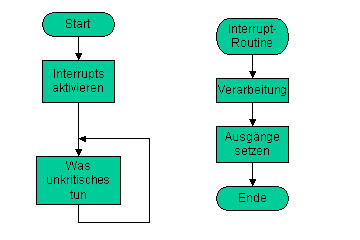
\includegraphics[width=0.8\textwidth]{rec/Interrupt_Programme.png}
			\caption[Interruptgesteuerter Programmablauf]{Interruptgesteuerter Programmablauf \hyperref[src:scout1]{[scout1]}}
			\label{InterruptgesteuerterProgrammablauf}
		\end{figure}
Der Programmablauf ist interruptgesteuert und folgt damit dem Modell in Abbildung \ref{InterruptgesteuerterProgrammablauf}.
			Dies hat den Vorteil, dass das Timing nicht mehr von der Länge der MainLoop abhängt und Vorgänge wie zum  Beispiel der Regelalgorithmus immer mit der selben Frequenz ausgeführt werden.
			In der Mainloop des Programms werden zeitunkritische Aufgaben erledigt, wie die LEDs der HMI zu aktualisieren.
			Interruptquellen des Programms sind:
			\begin{itemize}
				\item Timer  (Abschnitt \ref{subsubsec:Timer})
				\begin{itemize}
					\item[1.] Timer1, Compareregister B match
					\item[2.] Timer3, Compareregister A match
					\item[3.] Timer4, Compareregister A match
				\end{itemize}
				\item Pin Change Interrupts (Abschnitt \ref{subsubsec:PCINT})
				\begin{itemize}
					\item[4.] PCINT0\underline{ }vect
					\item[5.] PCINT1\underline{ }vect
					\item[6.] PCINT2\underline{ }vect
				\end{itemize}
				\item Analog Digital Converter
				\begin{itemize}
					\item[7.] ADC\underline{ }vect  (Abschnitt \ref{subsubsec:ADCINT})
				\end{itemize}

			\end{itemize}
%HIER WEITER
			\subsubsection{Timer}\label{subsubsec:Timer}
			Für die Funktion der Steuerung werden viele Timer benötigt.\\
			Da im Mikrocontroller allerdings nur begrenzt Hardwaretimer zur Verfügung stehen, ist deren Funktionalität in einem Softwaretimer nachgebildet.
			Dieser bezieht seinen Takt von dem  Hardwaretimer \glqq Timer4\grqq.
			Die Verwendung der Hard- sowie Softwaretimer kann der Tabelle \ref{tab:belegungTimer} entnommen werden.
				\begin{table}[ht]
					\begin{tabular}{|l|l|l|}
						\hline
						\textbf{Timer} & \textbf{Funktion}\\
						\hline
						\hline
						 & \\
						Hardwaretimer &\\
						\hline
						\hline
						Timer0 & Generierung der 2 PWM Kanäle für die Tiefsetzsteller\\
						\hline
						Timer1 & Auslösen der Analog Digital Wandlung\\
						\hline
						Timer2 & Ohne Verwendung\\
						\hline
						Timer3 & Trigger für Spannungsregelung\\
						\hline
						Timer4 & Trigger für Softwaretimer\\
						\hline
						\hline
						 & \\
						Softwaretimer &\\
						\hline
						\hline
						0..1 & Zeitmessung Abschnitt 3 (Nach dem Looping $\rightarrow$ Startlinie)\\
						\hline
						2..7 & Entprellen der Bahnsensoren\\
						\hline
						8..14 & Entprellen der HID Taster\\
						\hline
						15..16 & Ohne Verwendung\\
						\hline
						17 & Trigger für Zeitmessung Resettaster Visualisierung (langer Tastendruck)\\
						\hline
					\end{tabular}
					\caption{Belegung der Hard- sowie Softwaretimer}
					\label{tab:belegungTimer}
				\end{table}
			\subsubsection {Pin Change Interrupt}\label{subsubsec:PCINT}
			Wenn ein Auto auf, beispielsweise Sensor 0 (Bahn A, am Start), fährt, wird der Pegel kurze Zeit \emph{Low} und nach Verlassen des Sensors wieder \emph{High}.\\ Sensor 0 ist nach Tabelle \ref{tab:belegungpcint} an PCINT16 angeschlossen. Aus dem Datenblatt des Mikrocontrollers (ATmega2560) geht hervor, dass für die Pin Chage Interrupts, drei Interruptvektoren vorgesehen sind. Dabei besteht eine Zuordnung von jeweils immer 8 PCINT Pins an einen Interruptvektor. Diese Zuordnung beginnt bei dem Pin PCINT0 und PCINT0\underline{}vect. Durch das Überfahren des Autos über den Sensor, wird also das letzte Pin Change Interrupt, PCINT2\underline{ }vect, zweimal ausgelöst. In der Interrupt Service Routine (ISR) muss nun unterschieden werden, durch welchen Pin, das Interrupt ausgelöst wurde.
			Die Lösung dieses Problems ist gegeben, indem der Signalpegel der PCINT Pins in der letzten ISR gesichert wurden. Nun wird das aktuelle Eingangsbyte des Ports mit dem zuvor gespeicherten bitweise exklusiv-oder verknüpft.
Ist das Ergebnis der Verknüpfung nicht \glqq 0\grqq, entspricht die Stelle der logischen \glqq 1\grqq im Byte, der Nummer des PCINT Pins gezählt von dem ersten zugeordneten Pin des Interruptvektors. So ist das Ergebnis der exklusiv-oder Verknüpfung dieses Beispiels mit Sensor 0: $00000001$ da sich das nullte Bit verändert hat. 
In der ISR muss nun weiter, zwischen den zwei Möglichkeiten, unterschieden werden:
				\begin{itemize}
					\item \emph{High$\rightarrow$Low} Übergang
					\item \emph{Low$\rightarrow$High} Übergang
				\end{itemize}
			Hat ein \emph{High$\rightarrow$Low} Übergang stattgefunden, wird ein Event erzeugt und je nach PCINT Pin unterschiedlich behandelt.
			Bei einem \emph{Low$\rightarrow$High} Übergang, kann das Ereignis verworfen werden.

			Das Entprellen des Eingangs ist implementiert, indem nach dem Auslösen eines Events, die PCINT Funktion für den zugehörigen Pin deaktiviert wird, sodass dieser das Interrupt nicht mehr auslösen kann. Zusätzlich wird ein Softwaretimer gestartet, der die PCINT Funktion des Pins, nach dessen Ablauf wieder aktiviert. Mit diesem einfachen Prinzip wird sichergestellt, dass das Auto beim Überfahren des Sensors, das dementsprechende Event nur einmal triggert.
			Analog zu dem Sensor 0, ist dies für jeden Sensor sowie Taster implementiert. Die Belegung der benutzten Pin Change Interrupts kann Tabelle \ref{tab:belegungpcint} entnommen werden.
			\begin{table}[ht]
				\begin{tabular}{|l|l|l|}
					\hline
					Zugehörigkeit & Signal & Bezeichnung\\
					\hline
					\hline
					PCINT0\underline{ }vect & PCINT4 & Button: B-Automatik\\
					\hline
											& PCINT5 & Button: B-Manuell\\
					\hline
											& PCINT6 & Button: A-Automatik\\
					\hline
					\hline
					PCINT1\underline{ }vect & PCINT9 & Button: A-Reset\\
					\hline
											& PCINT10 & Button: B-Reset\\
					\hline
					\hline
					PCINT2\underline{ }vect & PCINT16 & Sensor: 0\\
					\hline
											& PCINT17 & Sensor: 1\\
					\hline
											& PCINT18 & Sensor: 2\\
					\hline
											& PCINT19 & Sensor: 3\\
					\hline
											& PCINT20 & Sensor: 4\\
					\hline
											& PCINT21 & Sensor: 5\\
					\hline
											& PCINT22 & Button: Reset/Shutdown Pi\\
					\hline
											& PCINT23 & Button: A-Manuell\\
					\hline
				\end{tabular}
				\caption{Belegung der Pin Change Interrupts}
				\label{tab:belegungpcint}
			\end{table}
			\subsubsection{Analog Digital Converter Interrupt}\label{subsubsec:ADCINT}
			Zum Betrieb des Zustandsautomats (Abbildung \ref{img:ADCMUX}) welcher den Multiplexer des ADC steuert ist ein Interrupt notwendig, welches ausgelöst wird, wenn der ADC eine Messung abgeschlossen hat. Dieser Automat ist genauer in Abschnitt \ref{subsec:ADC} beschrieben.

			%erklärung an diesem
	\subsection{Regler}
		\begin{figure}[ht]
			\centering
			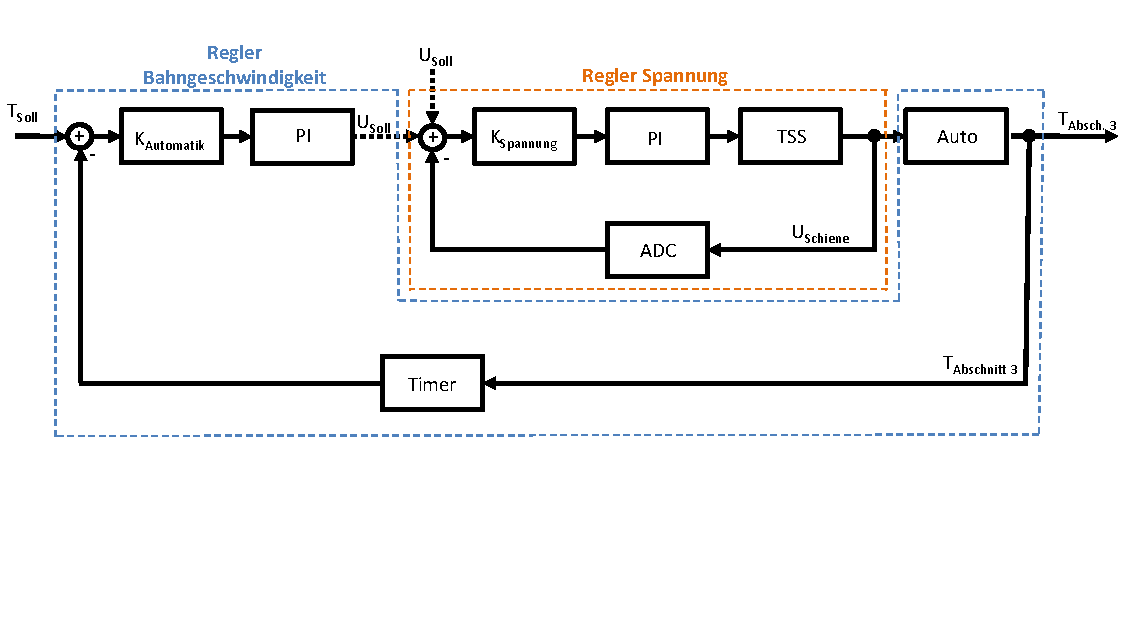
\includegraphics[width=\textwidth]{rec/Regler.pdf}
			\caption{Kaskadenreglung Bahngeschwindigkeit}
			\label{img:Regelung}
		\end{figure}
		Die Regelung für die Bahngeschwindigkeit ist als Kaskadenregelung (Abbildung \ref{img:Regelung}) ausgeführt.
		Dem Führungsregler wird eine konstante Sollzeit für Streckenabschnitt 3 vorgegeben. Dieser gibt nun, im Automatikmodus, die Sollspannung für den Folgeregler vor.
		Im manuellen Modus entspricht die Sollspannung einer skalierten Größe des jeweiligen Handreglers.
		Der Folgeregler hat als Stellgröße den Duty-Cycle des zugehörigen Tiefsetzstellers und regelt die Spannung auf der Schiene auf den gegebenen Wert.
		Der Regelalgorithmus des Spannungsreglers wird in festen Zeitabständen, vorgegeben durch OCR3 (Overflow Compare Register Timer3), zyklisch aufgerufen.
		Der Regelalgorithmus des Reglers der Bahngeschwindigkeit wird immer dann aufgerufen, wenn ein neuer Zeitwert für den Streckenabschnitt 3 vorliegt.
		Dieses Vorgehen ist durch die geringe Abtastrate des Führungsregles sehr störanfällig (Zum Beispiel wenn man das Auto in Streckenabschnitt 3 festgehalten wird), allerdings ist es die einzige Möglichkeit, einen solche Regelung mit den vorhandenen Sensoren zu realisieren. Die Bedingung für eine Kaskadenregelung (inner Regelkreis mindestens 10mal schneller als der Äußere) ist sicher eingehalten.\\
		Der Vorfaktor des Führungsreglers ist eher verhältnismäßig klein gewählt, um ein Überschwingen möglichst zu Verhindern, da dies bedeuten würde, dass das Auto die Strecke verlässt.
		Die gerade beschriebene Regelstrategie ist als solche nur im Automatik-Modus aktiv.\\
		Im manuellen Modus wird die Sollspannung direkt durch den Handregler vorgegeben.
		\newpage
	\subsection{Analog Digital Wandler}\label{subsec:ADC}

		Der Mikrocontroller des Arduinos (Atmega2560) hat bereits einen 10-bit Analog Digital Converter (ADC) auf dem Chip integriert, sodass auf einen externen Wandler, verzichtet wird.
		Da der Wandler immer nur eine Messung durchführen kann, hat der Hersteller einen Multiplexer (MUX) integriert, um zwischen den einzelnen ADC Pins (Kanälen), des Mikrocontrollers durchzuschalten.
		Die Belegung der ADC Pins ist in Tabelle \ref{tab:AnhangBelegungArduino} enthalten.

		Immer wenn die angestoßene Messung des ADC abgeschlossen ist, wird ein Interrupt ausgelöst.

		Die Steuerung des MUX erfolgt über ein Zustandsautomat (siehe Abbildung \ref{img:ADCMUX}), der immer dann ein Schritt weiter springt, wenn dieses Interrupt eintritt. In jedem Schritt des Automats, wird schematisch dasselbe durchgeführt:
		\begin{itemize}
		\item	Letzter gemessener Wert in zugehörige Variable speichern
		\item Nächste Messung vorbereiten (Multiplexer steuern und Messung anstoßen)
		\end{itemize}

		\begin{figure}[ht]
			\centering
			\includegraphics[width=0.3\textwidth]{rec/ADCAutomat.png}
			\caption[Zustandsautomat des MUX im ADC]{Zustandsautomat des MUX im ADC.\\Die Zustände(S0 bis S1) beschreiben, welcher ADC Pin des Mikrocontrollers gerade durch den MUX mit dem ADC verbunden ist. Die Transitionsbedingung (links) beschreibt das Ereignis, mit dem man von einem Zustand in den Nächsten wechselt. Ein Punkt markiert den Schritt in den Initialzustand (S0) des Automats und ein Pfeil einen Sprung zu einem darunter definierten Zustand.}
			\label{img:ADCMUX}
		\end{figure}

\subsection{PWM Generierung Tiefsetzsteller}\label{subsec:PWM}


\begin{figure}[htp]
	\centering
	\subcaptionbox{Zustandsautomat PWM Generierung
        \label{fig:PWMGENAut}}
        {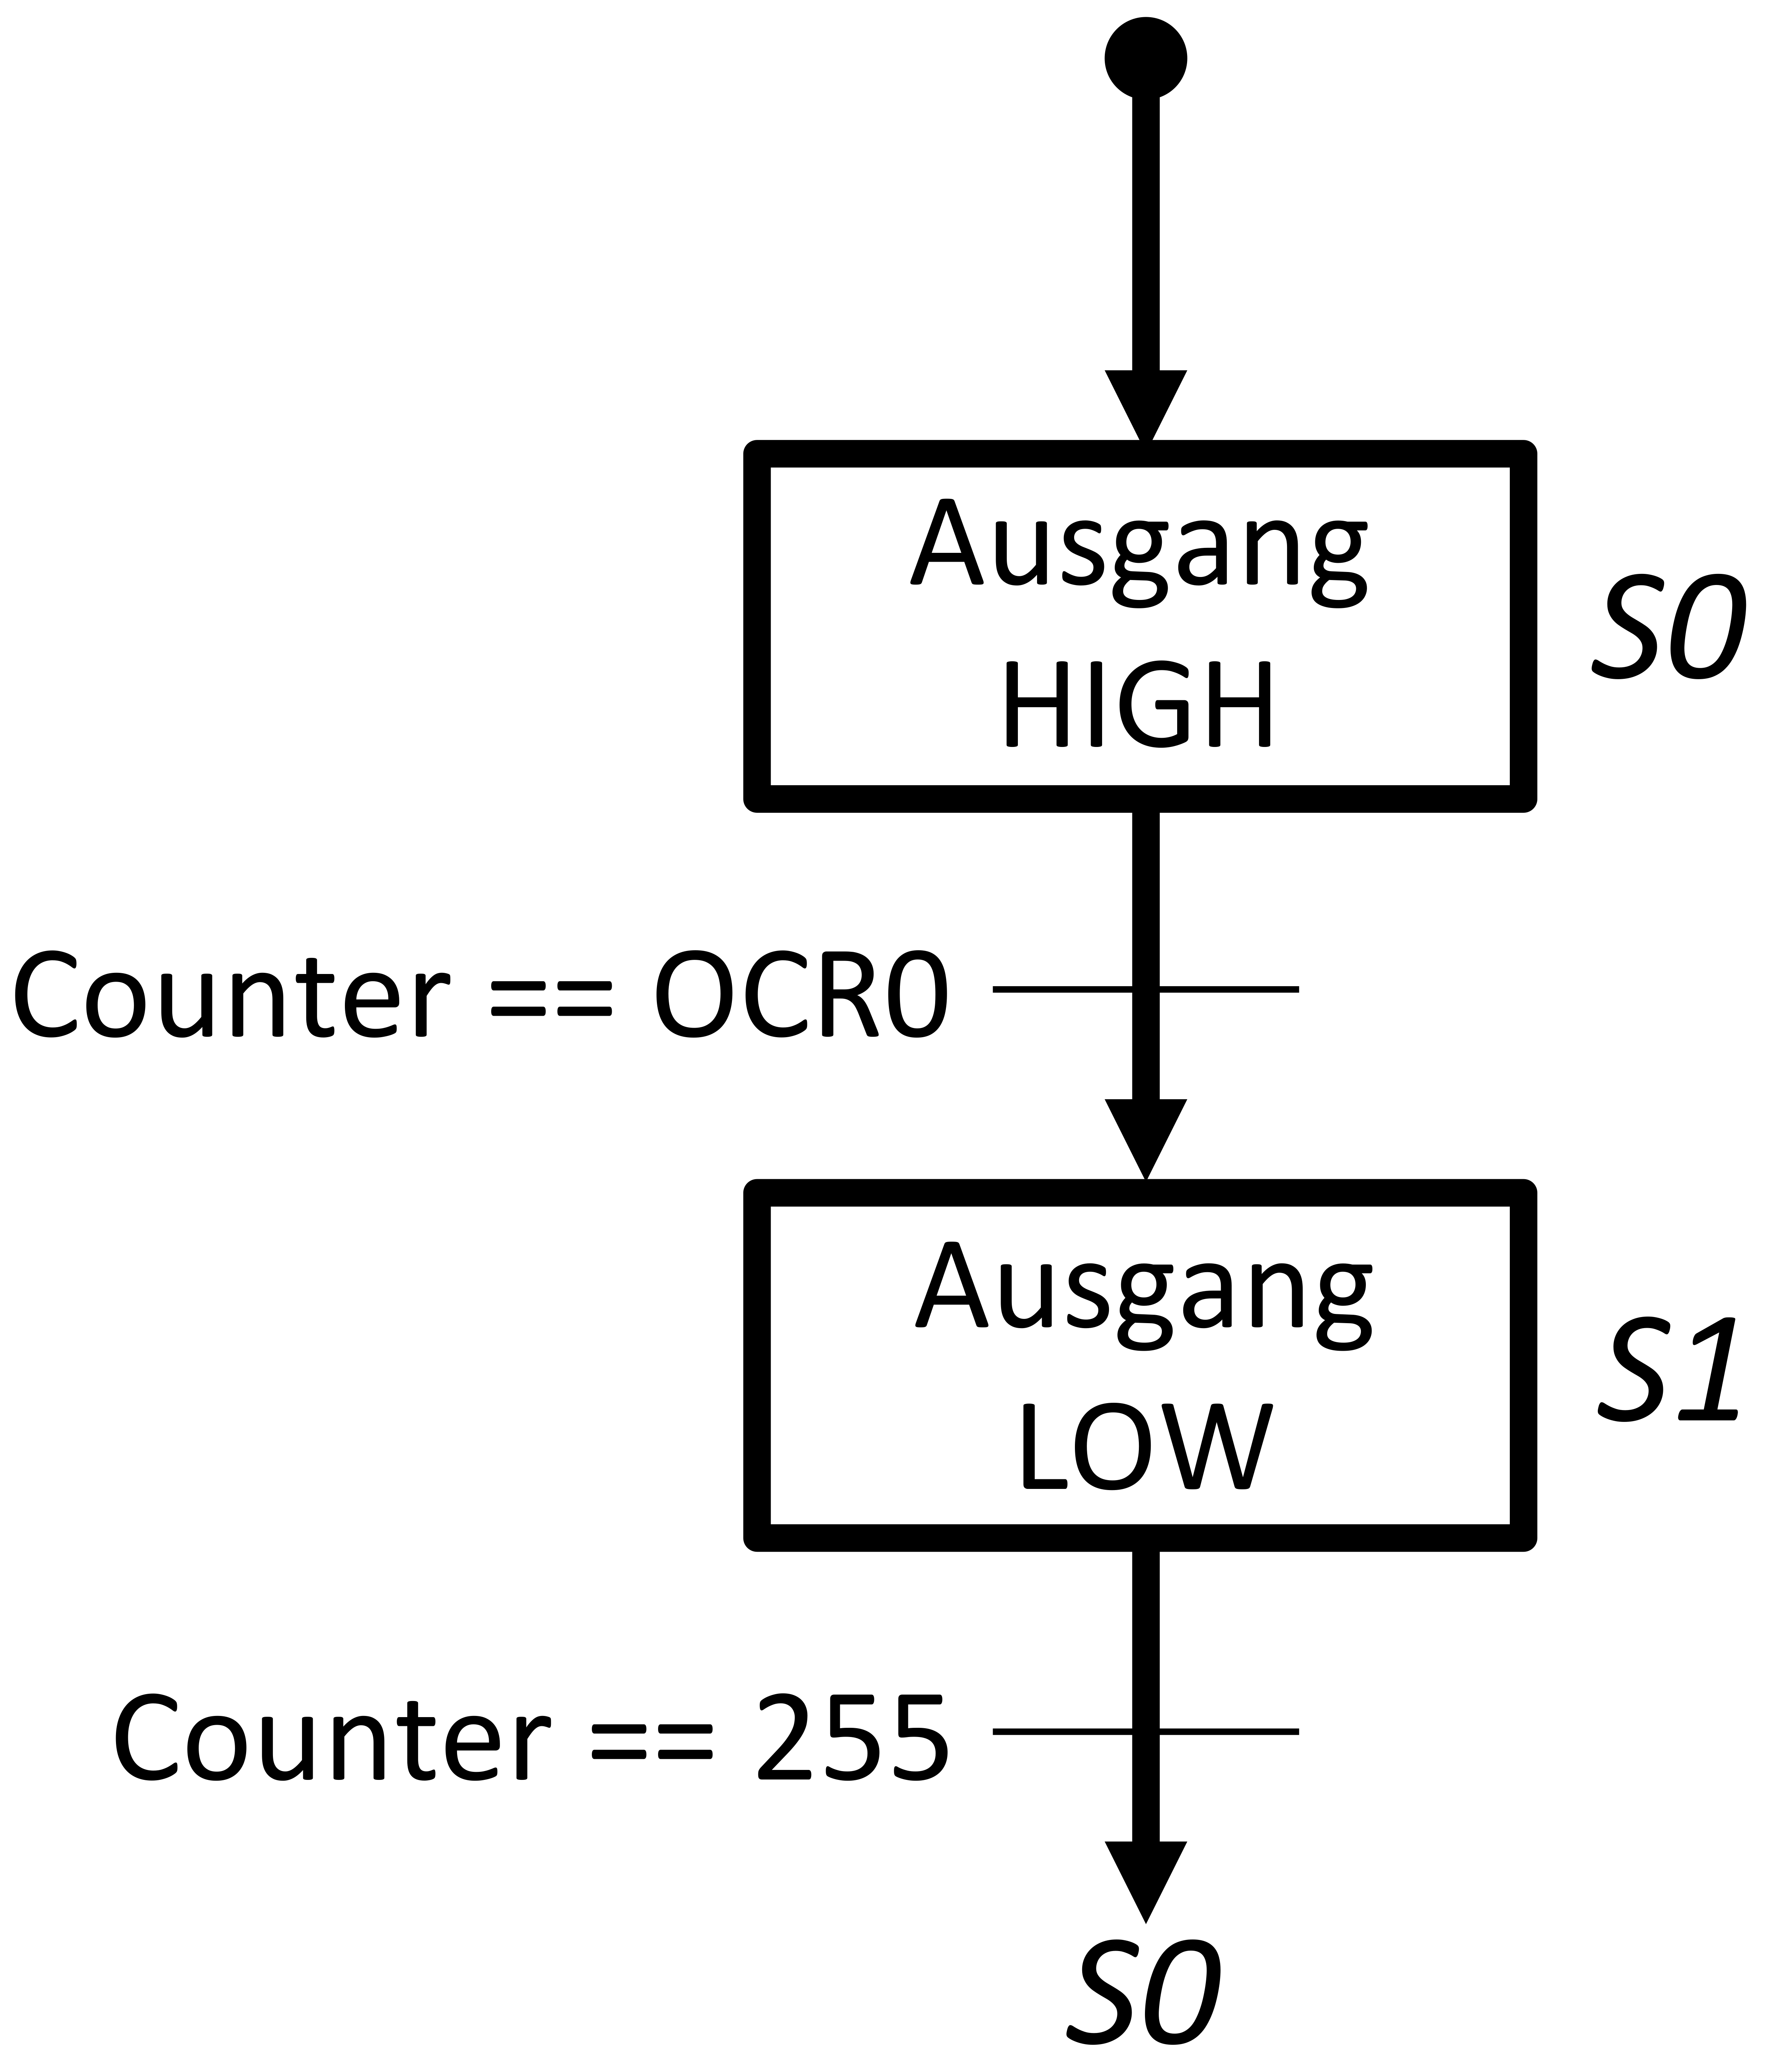
\includegraphics[width=0.34\textwidth]{rec/zustandsautomatPWM.png}}
        \hfill
  \subcaptionbox{Ausgang PWM Pin als Funktion des Zählerstands
        \label{fig:PWMGENFX}}
        {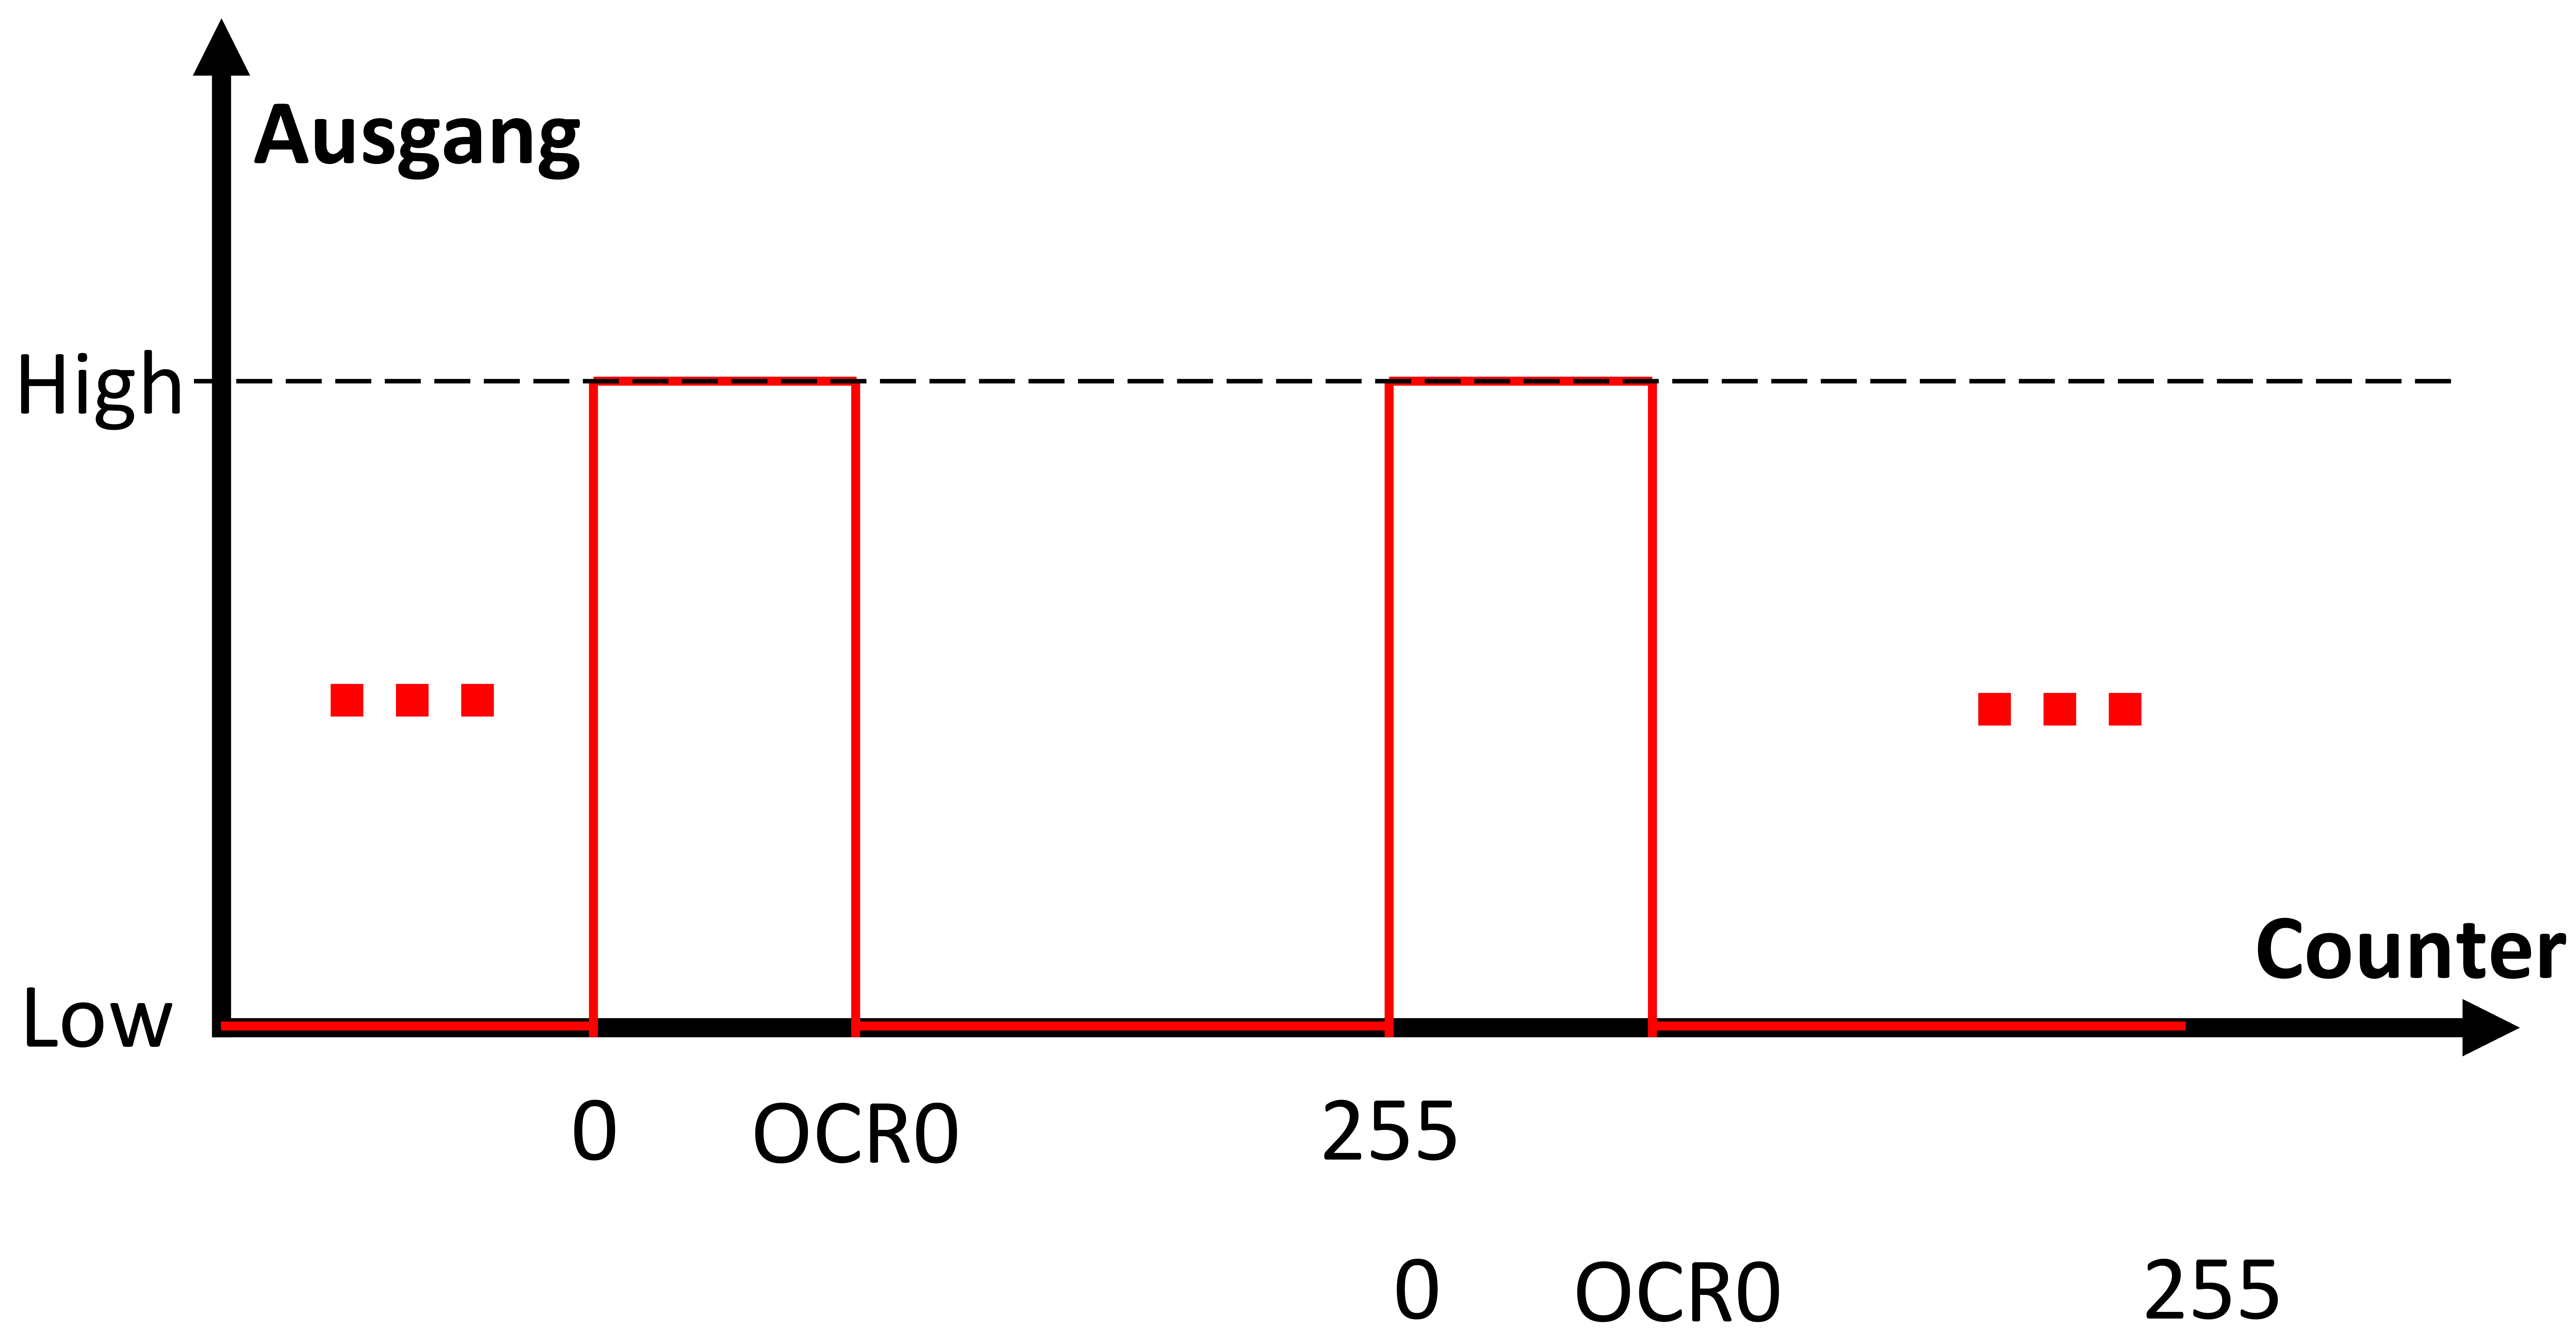
\includegraphics[width=0.64\textwidth]{rec/graphPWM.png}}
    \caption{Zustandsautomat des Timers zur PWM Generierung, sowie resultierendes Ausgangssignal bei konstantem Dutycycle.}


\end{figure}




Wie aus Abbildung \ref{fig:PWMGENFX} hervorgeht, ist das PWM Signal direkt eine Funktion des aktuellen Zählerstands von Timer0, sowie dem Inhalt des jeweiligen Overflow Compare Registers OCR0A/B.
Die PWM Generierung ist durch den Mikrocontroller in Hardware implementiert und muss lediglich aktiviert werden. Die Konfiguration dieser PWM Generierung ist in der Funktion initTimer implementiert und wird einmal zu Programmstart aufgerufen. Der Hardwaretimer setzt nun den jeweiligen Pin beim Überlauf des 8-bit Timers (Wert 0) auf High-Pegel und beim Erreichen des Wertes im OCR0AB Registers ( zum Beispiel  bei DutyCycle = 50\% OCR0A = 127 ) auf Low-Pegel.
Dieses Verhalten des Hardwaretimers ist zur Veranschaulichung nochmal in Abbildung  \ref{fig:PWMGENAut} als Zustandsautomat dargestellt.



\chapter{Bedienungsanleitung}
\section{Einschalten}
	Die Anlage muss zum Einschalten lediglich mit der Netzversorgung verbunden werden. Sobald die Anlage Spannung hat, bootet der RaspberryPi selbständig und startet die Visualisierung. Ab diesem Punkt ist die Carrera Bahn betriebsbereit und im Modus manuelles Fahren (Abschnitt \ref{subsec:ManuellesFahren}).
\section{Betrieb}
	\begin{figure}[ht]
		\centering
		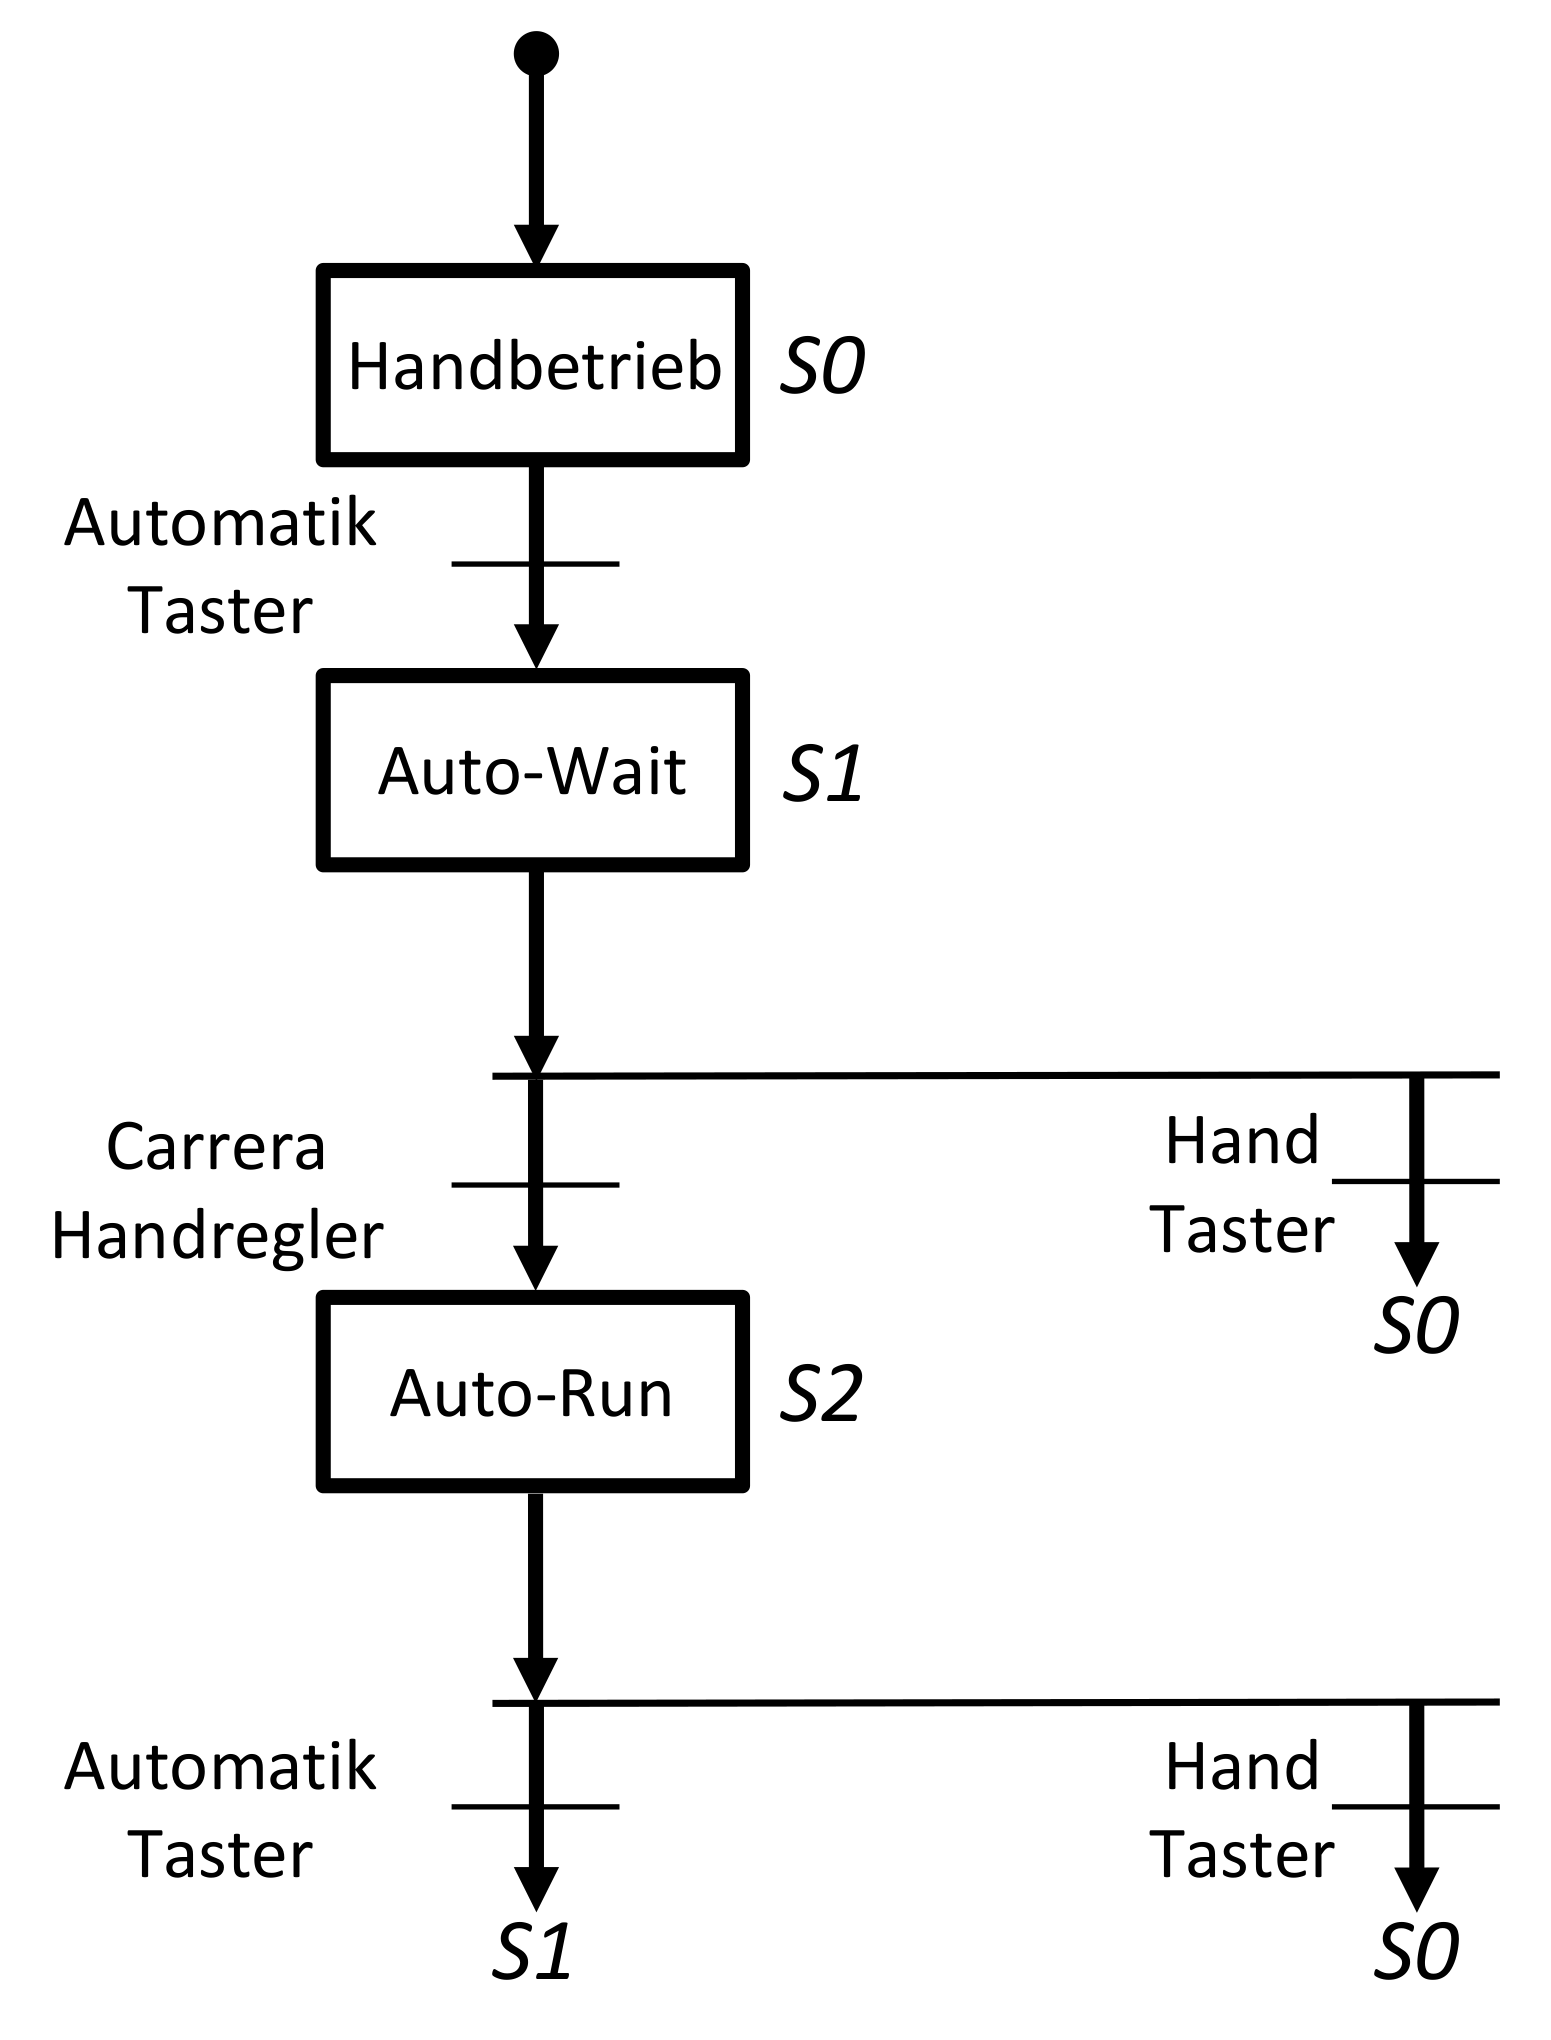
\includegraphics[width=0.5\textwidth]{rec/modiAuswahl.png}
		\caption[Zustandsautomat zum Wechsel der Betriebsmodi]{Zustandsautomat zum Wechsel der Betriebsmodi.\\Durch den \glqq HMI Taster Auto \grqq der jeweiligen Bahn, kann der Nutzer immer in den \glqq Auto-Wait\grqq Zustand (S1) wechseln, in dem das Auto hält. Von diesem Zustand aus, kann der Nutzer die Bahn durch Betätigung des Handreglers, in den \glqq Auto-Run\grqq Zustand (S2) versetzten und das Auto fährt anschließend selbständig. Aus jedem Zustand kann der Nutzer mit dem \glqq HMI Taster Manuell \grqq, die Bahn in den Handbetrieb versetzten und das entsprechende Auto mit dem Handregler manuell steuern.}
		\label{img:Betriebsmodi}
	\end{figure}
	Die Carrera Bahn beherrscht 2 Modi.
	\begin{itemize}
		\item Manuelles Fahren
		\item Automatisiertes Fahren
	\end{itemize}
	Die Modi können unabhängig voneinander auf beiden Bahnen gewählt werden, sodass man zum Beispiel manuell gegen ein automatisiertes Fahrzeug antreten kann. Die Wahl eines dementsprechenden Modus wird durch eine Led über, beziehungsweise unter, des jeweiligen Tasters des gewählten Modus signalisiert. Außerdem kann die Energieversorgung jeder Bahn mit dem entsprechenden Wechselschalter ausgewählt werden. Unabhängig des gewählten Modus, wird in der Visualisierung die Zeit der 2 Abschnitte, sowie die Rundenzeit angezeigt. Nach 30 Runden ist das Rennen vorbei und die Visualisierung wird statisch.
	Der Wechsel zwischen den Modi findet nach Abbildung \ref{img:Betriebsmodi} statt und ist in den jeweiligen Abschnitten genauer erklärt.
	\subsection{Manuelles Fahren}\label{subsec:ManuellesFahren}
		Im Modus Manuelles Fahren kann das Fahrzeug konventionell über die orginalen Carrera Handregler gesteuert
		werden.
\newpage
	\subsection{Automatisiertes Fahren}
		Der Automatisierte Modus ist aufgeschlüsselt in 2 Zustände:
		\begin{itemize}
			\item Auto-Wait
			\item Auto-Run
		\end{itemize}
		\subsubsection{Auto-Wait}
		Immer wenn in den Modus des Automatisierten Fahrens gewechselt wird, startet die Steuerung in
		Auto-Wait und das Auto steht.
		Durch kurzes durchdrücken des zugehörigen Handreglers, wechselt das Auto in den Auto-Run Zustand.
		\subsubsection{Auto-Run}
			Im Auto-run Zustand fährt das Auto selbständig. Durch die Regelung der mittleren Geschwindigkeit des langsamen Streckenabschnitts, braucht das Auto einige Runden um die optimale Spannung, für diese Geschwindigkeit zu finden.

			In der Visualisierung ist die Strecke von der Startlinie bis vor den Looping in Streckenabschnitt 1 zusammengefasst.
			Der Rest einer Runde (vor dem Looping bis zur Startlinie) bildet Streckenabschnitt 2.
\section{Ausschalten}
Um die Anlage ordnungsgemäß herunterzufahren, ist der Reset Taster am HMI (Abbildung \ref{img:hid} - Reset Visualisierung) mindestens 5 Sekunden gedrückt zu halten.
Nun muss man warten bis der RaspberryPi komplett heruntergefahren ist. Dies ist daran zu erkennen, dass die grüne Led auf dem RaspberryPi nichtmehr blinkt und der Bildschirm in den Standby-Modus schaltet.
\chapter{Zusammenfassung}
Die Zu Beginn definierten Ziele der Projektarbeit wurden durch das neue Steuer-/Regelkonzept, sowie eine neue Hardware Architektur, fast alle erreicht. Lediglich die Robustheit der Anlage ist ist nicht vollsändig gegeben, da gelegentlich ein Auto im Looping herunterfällt.
Durch längere Tests und Analyse der Fehlerbilder, hat sich herausgestellt, dass dies kein Problem der Automatisierung und Regelung selbst darstellt, sondern vielmehr der schlechten Qualität der zugekauften Carrera Bahn.
Man hat herausgefunden dass im Looping die Stromschiene auf der Bahn, ein wenig in der Oberfläche versenkt ist und der Übergang zwischen den zusammengesteckten Streckenstücken einen unstetigen Verlauf hat. Dadurch ergibt sich eine Diskontinuität des Stroms durch den Antrieb des Fahrzeugs im Looping, was zu Geschwindigkeitsverlust, sowie letztendlich zum Absturz des Fahrzeugs führt. Biegt man nun die Strombürsten des Fahrzeugs weiter in Richtung Schiene um die schlechte Mechanische Beschaffenheit auszugleichen, taucht die Führungsnase nicht mehr weit genug in die Bahn ein und das Fahrzeug fliegt aus der Kurve oder triggert die Sensoren nichtmehr verlässlich.
Ein weitere Randbedingung für die Realisierung war dass die Automatisierung unabhängig von der länge der Strecke funktionieren sollte.
Aufgrund dieser Forderung musste die Funktionalität, das Auto auf der Geraden zu beschleunigen verworfen werden, da dies nun nichtmehr in Abhängigkeit einer konstante Zeit realisiert werden kann. Als weiterführende Verbesserung könnte man zusätzliche Sensoren vor der Kurve zum abremsen einbauen.
Ein weiteren Vorschlag zur Weiterarbeit wäre die Energieversorgung des RaspberryPi, sowie des Arduino auch autark über die Solarpanels zu ermöglichen.




\chapter{Quellenverzeichnis}
Scout1. (September 2004). Interrupt Programme.gif – Mikrocontroller.net. 
\\Von Mikrocontroller.net: \href{https://www.mikrocontroller.net/articles/Datei:Interrupt_Programme.gif}
{\url{https://www.mikrocontroller.net/articles/Datei:Interrupt_Programme.gif}} abgerufen \label{src:scout1}
\chapter{Anhang}


	\begin{table}[H]
	\centering
		\begin{tabular}{|l|l|}
			\hline
			\textbf{Sub-D Pin} &\textbf{Funktion}\\
			\hline
			\hline
			1 & VCC (5V)\\
			\hline
			2 & GND\\
			\hline
			3 & -\\
			\hline
			4 & -\\
			\hline
			5 & -\\
			\hline
			6 & Sensor 0\\
			\hline
			7 & Sensor 1\\
			\hline
			8 & Sensor 2\\
			\hline
			9 & Sensor 3\\
			\hline
			10 & Sensor 4\\
			\hline
			11 & Sensor 5\\
			\hline
			12 & Schiene A - Plus\\
			\hline
			13 & Schiene A - Minus\\
			\hline
			14 & Schiene B - Plus\\
			\hline
			15 & Schiene B - Minus\\
			\hline
		\end{tabular}
		\caption{Pinbelegung der Sub-D Buchse auf dem HMI}
		\label{tab:AnhangBelegungSUBD}
	\end{table}

	\begin{table}[H]
	\centering
		\begin{tabular}{|l|l|}
			\hline
			\textbf{Raspberry Pin} &\textbf{Funktion}\\
			\hline
			\hline
			1 & VCC MCU (3V3)\\
			\hline
			2 & VCC Input (5V)\\
			\hline
			3$\rightarrow$5 & -\\
			\hline
			6 & GND Input\\
			\hline
			7 & -\\
			\hline
			8 & -\\
			\hline
			9 & -\\
			\hline
			10 & RXD Uart\\
			\hline
			11$\rightarrow$40 & -\\
			\hline
		\end{tabular}
		\caption{Pinbelegung GPIO RaspberryPi}
		\label{tab:AnhangBelegungRPI}
	\end{table}

	\begin{table}[hb]
		\begin{tabular}{|l|l|l|}
			\hline
			\textbf{Arduino Pin} & \textbf{Atmel Pin} &\textbf{Funktion}\\
			\hline
			\hline
			0 &  & Ohne Funktion\\
			\hline
			1 &  & Ohne Funktion\\
			\hline
			2 &  & Ohne Funktion\\
			\hline
			3 &  & Ohne Funktion\\
			\hline
			4 & OC0B & PWM Tiefsetzsteller Schiene B\\
			\hline
			5 &  & Ohne Funktion\\
			\hline
			6 &  & Ohne Funktion\\
			\hline
			7 &  & Ohne Funktion\\
			\hline
			8 &  & Ohne Funktion\\
			\hline
			9 &  & Ohne Funktion\\
			\hline
			10 & PCINT4 & Taster HID \glqq Schiene B - Automatik\grqq \\
			\hline
			11 & PCINT5 & Taster HID \glqq Schiene B - Manuell\grqq \\
			\hline
			12 & PCINT6 & Taster HID \glqq Schiene A - Automatik\grqq \\
			\hline
			13 &  OC0A & PWM Tiefsetzsteller Schiene A\\
			\hline
			14	& PCINT10	& Taster HID \\
				&		& \glqq Schiene B - Reset Regler Bahngeschwindigkeit\grqq \\
			\hline
			15 	& PCINT9 	& Taster HID \\
				&		& \glqq Schiene A - Reset Regler Bahngeschwindigkeit\grqq \\
			\hline
			16 &  & Ohne Funktion\\
			\hline
			17 &  & Ohne Funktion\\
			\hline
			18 &  & Serielle Verbindung zu RaspberryPi\\
			\hline
			19$\rightarrow$45 &  & Ohne Funktion\\
			\hline
			46 & PL3 & HID LED \glqq Schiene B - Manuell\\
			\hline
			47 & PL2 & HID LED \glqq Schiene B - Automatik\\
			\hline
			48 & PL1 & HID LED \glqq Schiene A - Manuell\\
			\hline
			49 & PL0 & HID LED \glqq Schiene A - Automatik\\
			\hline
			A1$\rightarrow$A0 & ADC1$\rightarrow$ADC0 & Shunt Tiefsetzsteller Schiene A\\
			\hline
			A3$\rightarrow$A2 & ADC3$\rightarrow$ADC2 & Shunt Tiefsetzsteller Schiene B\\
			\hline
			A4 & ADC4 & Spannung Schiene A\\
			\hline
			A5 & ADC5 & Spannung Schiene B\\
			\hline
			A6 & ADC6 & Carrera Handregler Schiene A\\
			\hline
			A7 & ADC7 & Carrera Handregler Schiene B\\
			\hline
			A8 & PCINT16 & Sensor 0 (Schiene A - Startlinie)\\
			\hline
			A9 & PCINT17 & Sensor 1 (Schiene A - vor dem Looping)\\
			\hline
			A10 & PCINT18 & Sensor 2 (Schiene A - nach dem Looping)\\
			\hline
			A11 & PCINT19 & Sensor 3 (Schiene B - Startlinie)\\
			\hline
			A12 & PCINT20 & Sensor 4 (Schiene B - vor dem Looping)\\
			\hline
			A13 & PCINT21 & Sensor 5 (Schiene B - nach dem Looping)\\
			\hline
			A14 & PCINT22 & Taster HID \glqq Reset Rundenzeit Visualisierung\grqq \\
			\hline
			A15 & PCINT23 & Taster HID \glqq Schiene A - Manuell\grqq \\
			\hline
		\end{tabular}
		\caption{Pinbelegung des Arduino}
		\label{tab:AnhangBelegungArduino}
	\end{table}


\end{document}
